\documentclass[10pt]{scrartcl}

\usepackage[ngerman]{babel}
%%% Für PDFLatex
%\usepackage[utf8]{inputenc}
%\usepackage[T1]{fontenc}
%%% Für XeLaTeX
\usepackage{fontspec}
\setmainfont{DejaVu Sans}
%%%
\usepackage{graphicx}
\usepackage[
	a4paper,
	top=1cm,
	bottom=2cm,
	right=2cm,
	left=2.5cm]{geometry}
\usepackage{booktabs}
\usepackage{tabularx}
\usepackage[table]{xcolor}
\usepackage{hyperref}

\title{Designreport Embedded Software Development}
\subtitle{Erstellen einer Wetterstation mit digitalem Thermometer und Hygrometer, sowie Uhranzeige}
\author{Marco Gabrecht (271949)\\Matthias Hinrichs (290849)\\Sven Marquardt (240747)}
\date{18.01.2018}

\begin{document}
\maketitle
\vfill
\begin{center}
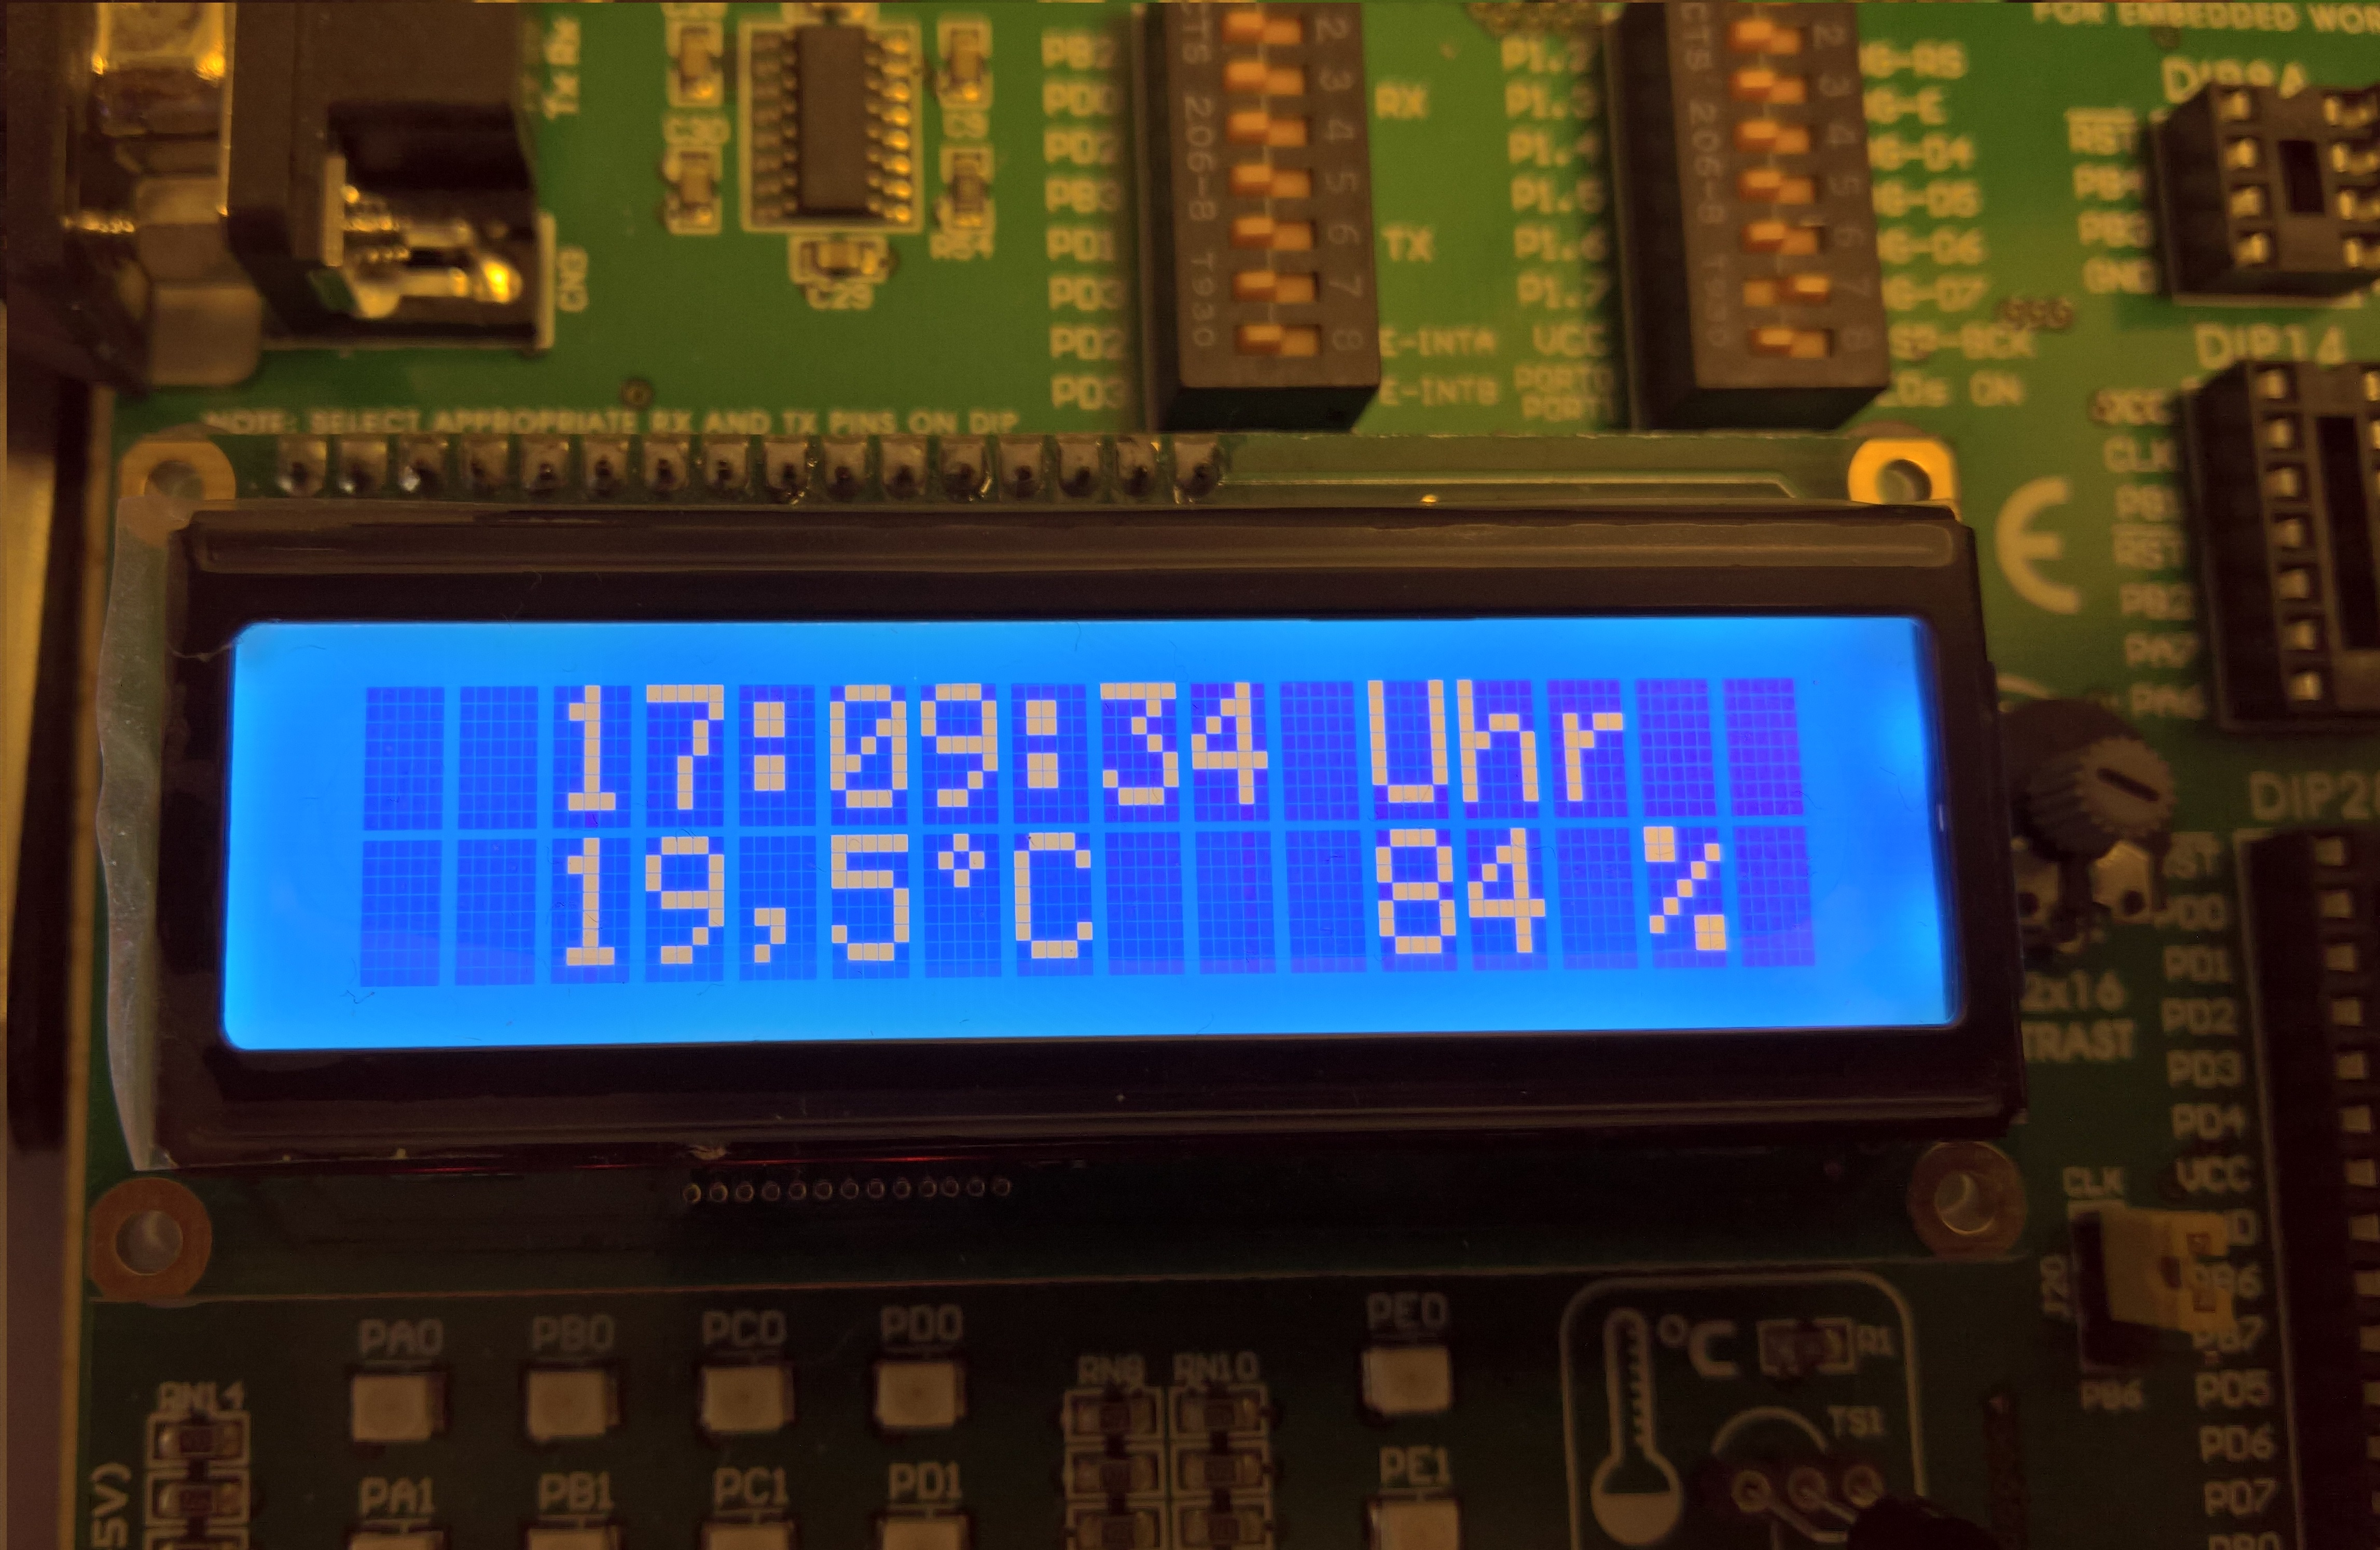
\includegraphics[width=0.9\textwidth]{img/designreport-title-hq.jpg}
\end{center}
\vfill
\newpage
\tableofcontents
\newpage
\section{Vorwort}
In diesem Designreport gehen wir darauf ein wie wir, die Wetterstation implementiert haben. Es werden sowohl die Entwicklungsentscheidungen, als auch die getroffenen Annahmen und die Implementierung beschrieben. Zudem enthält dieser Report die Komponentenbeschreibungen.
\section{Anforderungen}
An das Projekt wurden folgende Anforderungen gestellt
\begin{enumerate}
\item Eine einstellbare Uhr im 24-Stunde-Format mit Sekundenanzeige
\item Auslesen eines DS1820-Temperatursensors
\item Auslesen eines Potentiometers und Interpretation als relative Luftfeuchtigkeit
\item Ausgabe alle Werte auf einem LCD-Display
\item Sinnvolle Genauigkeiten und Aktualisierungsintervalle
\item Vier verschiedene Anzeigeoptionen
\item Geeignetes Menü zur Konfiguration
\end{enumerate}
\section{Getroffene Annahmen}
Wir haben folgende Annahmen im Projekt getroffen:
\begin{enumerate}
\item Die geeignete Zeit bei dem Anzeigewechsel von \textit{Nur Uhrzeit} und \textit{Temperatur und Luftfeuchte} ist 10 Sekunden.
\item Da nur ein Sensor angeschlossen ist, kann beim One-Wire der Skiprom-Befehl verwendet werden.
\end{enumerate}
\section{Begründung wesentlicher Entwurfsentscheidungen}
Der AD-Wandler wird alle 5 Sekunden und der Temperatursensor alle 9 Sekunden ausgelesen. Diese Intervalle wurden gewählt, damit die Messungen nicht so häufig gleichzeitig stattfinden. Die Berechnung der Temperatur wird mit Festkommazahlen durchgeführt, damit auf Fließkommazahlen verzichtet werden kann. Das Keypad 4x4 wurde nicht benutzt, da eine Bedienung durch die Pfeiltasten mit Enter und Cancel vollkommen ausreicht und das JTAG-Interface nutzbar bleibt. Bei der Initialisierung des AD-Wandlers wird eine erste Wandlung durchgeführt, deren Ergebnis verworfen wird. Dies geschieht, weil die erste Messung nach der Initialisierung länger dauert. Die Tasten wurden durch einen Timer entprellt, so dass die Eingabe nach dem Drücken einer Taste ignoriert wird. Nach etwa 75ms ist die Eingabe wieder entsperrt. Wenn ein error passiert beim lesen der Temperatur weil der CRC check fehlschlägt, wird dieser Wert verworfen und das LCD nicht aktualisiert.
\section{Überblick Funktionsumfang und Limitationen}
Alle Module inkludieren die Header-Datei \textit{Global.h}. Alle Module, die etwas auf dem LCD-Display anzeigen inkludieren die Header-Datei \textit{lcd.h}.
\subsection{One-Wire}
Beinhaltet die Header-Datei \textit{ds18s20.h} und \textit{onewire.h}. \textit{Onewire.h} beinhaltet alle Funktionen um auf dem One-Wire auf Bitebene zu interagieren. \textit{Ds18s20.h} enthält alle Funktionen um Temperatur lesen bzw anzeigen zu können.
\subsection{LCD}
Beinhaltet die Header-Datei \textit{lcd.h}. Diese beinhaltet alle Funktionen um mit dem LCD zu interagieren.
\subsection{Clock}
Beinhaltet die Header-Datei \textit{clock.h}. Kann die Uhrzeit auf dem LCD-Display anzeigen und die Zeit einstellen.
\subsection{ADC}
Beinhaltet den Header \textit{adc.h} und \textit{hygro.h}. \textit{Adc.h} dient dazu den AD-Wandler auslesen zu können und zu initialisieren. \textit{Hygro.h} wandelt die Ausgabe des ADC in Werte um die als Luftfeuchtigkeit dargestellt werden können.
\subsection{Main}
Beinhaltet die Datei \textit{Aufgabe2.c}. Implementiert die gesamte Menüführung und kommuniziert mit den einzelnen Modulen für die Darstellungen.
\subsection{Global}
Die \textit{Global.h} Datei beinhaltet Einstellungen zu den Ports, Pins und DDRs. Außerdem inkludiert diese die Header-Datei \textit{delay.h} mit \textit{F\_CPU} um diese allen anderen Modulen zur Verfügung zu stellen mit der richtigen CPU-Geschwindigkeit.
\section{Beschreibung der Implementierung}
\subsection{One-Wire}
\subsubsection{temp\_display()}
Zum Anzeigen der Temperatur wird die Funktion \textit{temp\_display(uint8\_t row)} aufgerufen. Mit dem Parameter \textit{row} kann gesteuert werden in welcher Zeile die Temperatur angezeigt werden soll.
\subsubsection{ds18s20\_read\_temperature()}
Zum Auslesen der Temperatur wird die Funktion \textit{ds18s20\_read\_temperature()} aufgerufen. Diese sendet das Kommando \texttt{COMMAND\_CONVER\_T}. Der danach konvertierte Wert im Scratchpad wird ausgelesen und mit dem CRC verifiziert. Wurde der Wert durch die Übertragung kompromittiert hat die Variable \textit{status\_read\_temperature} den Wert 1, ansonsten den Wert 0.
\subsubsection{ds18s20\_temperature\_as\_string()}
Mit \textit{ds18s20\_read\_temperature()} gelesene Werte können mit der Funktion\\ \textit{ds18s20\_temperature\_as\_string()} in einen String gewandelt werden, der auf dem LCD-Display ausgegeben werden kann.
\subsection{LCD}
\subsubsection{lcd\_init()}
Die Funktion \textit{lcd\_init()} wird aufgerufen um das LCD-Display zu initialisieren. Hier wird der 4-Bit-Modus aktiviert, das Display auf zwei Zeilen mit 16 Zeichen der Größe 5x7 eingestellt das Blinken der aktuellen Position und des Cursors, sowie das automatische Shiften beim Schreiben deaktiviert.
\subsubsection{lcd\_clear()}
Die Funktion \textit{lcd\_clear()} löscht das Display.
\subsubsection{lcd\_cursor\_home()}
Die Funktion \textit{lcd\_cursor\_home()} setzt die DDRAM-Adresse auf 0 und setzt ein eventuell geshiftetes Display zurück in den Normalzustand.
\subsubsection{lcd\_set\_cursor()}
Die Funktion \textit{lcd\_set\_cursor(uint8\_t row, uint8\_t col)} setzt den Cursor an die durch die Parameter vorgegebene Stelle, indem die DDRAM-Adresse entsprechend gesetzt wird.
\subsubsection{lcd\_send\_nibble(uint8\_t nibble)}
Die Funktion \textit{lcd\_send\_nibble()} sendet das obere Nibble des Parameters an das LCD-Display.
\subsubsection{lcd\_send\_char()}
Die Funktion \textit{lcd\_send\_char(uint8\_t character)} sendet das als Parameter übergebenen Zeichen an das LCD-Display.
\subsubsection{lcd\_send\_string()}
Die Funktion \textit{lcd\_send\_string(const char *string)} sendet einen als Parameter übergebenen String mit Hilfe der Funktion \textit{lcd\_send\_char()} an das LCD-Display.
\subsubsection{lcd\_display\_string\_shift()}
Die Funktion \textit{lcd\_display\_string\_shift(const char *string, uint8\_t row)} sendet einen als Parameter übergebenen String mit Hilfe der Funktion \textit{lcd\_send\_string()} an das LCD-Display. Dabei wird entsprechend der Länge des Strings der Cursor so positioniert, dass der String zentriert dargestellt wird oder mit Hilfe der Funktion \textit{lcd\_shift\_left()} das Display so geshifted, dass der String als Lauftext erscheint.
\subsubsection{lcd\_send\_command()}
Die Funktion \textit{lcd\_send\_command(uint8\_t command)} sendet ein als Parameter übergebenes LCD-Kommando in zwei Nibble zerlegt an das LCD-Display. Das obere Nibble wird dabei zuerst gesendet.
\subsubsection{lcd\_send\_enable\_pulse()}
Die Funktion \textit{lcd\_send\_enable\_pulse()} sendet einen kurzen Puls an den \texttt{LCD\_E\_PIN} des LCD-Displays. 
\subsubsection{lcd\_shift\_left()}
Die Funktion \textit{lcd\_shift\_left(uint8\_t x)} führt die durch den Parameter übergebene Anzahl an Linksshiftoperationen des LCD-Displays durch. Diese werden durch ein über einen Timer gesetztes Flag verzögert um eine lesbare Darstellung auf dem LCD-Display zu gewährleisten. Die Shiftoperationen können durch ein weiteres Flag abgebrochen werden.
\subsection{Clock}
\subsubsection{clock\_display()}
Die Funktion \textit{clock\_display(uint8\_t row, uint8\_t blink\_pos)} zeigt mit Hilfe der Funktion\\ \textit{lcd\_display\_string\_shift()} die Uhrzeit auf dem LCD-Display an. Mit dem Paramter \textit{row} kann gesteuert werden in welcher Zeile die Uhrzeit angezeigt werden soll. Mit dem Parameter \textit{blink\_pos} wird gesteuert, ob die Stunden, die Minuten oder keins von beiden blinken soll. Durch ein Timergesteuertes Flag wird dann entsprechend der Teil des erstellten Strings durch Leerzeichen ersetzt. Im erstellten String werden je nach Stellenanzahl der Zeitvariablen führende Nullen hinzugefügt.
\subsubsection{clock\_hour\_inc()}
Die Funktion \textit{clock\_hour\_inc()} erhöht die Variable \textit{uint8\_t hours}. Sollte die Variable dadurch größer als \(23\) sein, so wird sie auf \(0\) gesetzt.
\subsubsection{clock\_hour\_dec()}
Die Funktion \textit{clock\_hour\_dec()} verringert die Variable \textit{uint8\_t hours}. Sollte die Variable dadurch größer als \(23\) sein, so wird sie auf \(23\) gesetzt.
\subsubsection{clock\_min\_inc()}
Die Funktion \textit{clock\_min\_inc()} erhöht die Variable \textit{uint8\_t minutes}. Sollte die Variable dadurch größer als \(59\) sein, so wird sie auf \(0\) gesetzt.
\subsubsection{clock\_min\_dec()}
Die Funktion \textit{clock\_min\_inc()} erhöht die Variable \textit{uint8\_t minutes}. Sollte die Variable dadurch größer als \(59\) sein, so wird sie auf \(59\) gesetzt.
\subsection{ADC}
\subsubsection{adc\_init()}
Die Funktion \textit{adc\_init()} konfiguriert den AD-Wandler.
\subsubsection{adc\_read()}
Die Funktion \textit{adc\_read()} wird genutzt um eine AD-Wandlung zu starten und anschließend nur das High-Byte auszulesen. Dadurch werden die unteren zwei Bits des Ergebnisses verworfen und die Auflösung auf 8-Bit verringert.
\subsubsection{hygro\_display()}
Die Funktion \textit{hygro\_display()} liest einen Wert vom AD-Wandler ein und skaliert ihn mit dem \textit{HYGRO\_MAP\_FACTOR} in den Bereich von \(0\)-\(100\). Im erstellten String werden je nach Stellenanzahl des Messwertes führende Leerzeichen hinzugefügt um eine stets gleiche Stringlänge zu gewährleisten.
\subsection{Main}
Jeder Menüpunkt und jeder Displayanzeigemodus hat eine eigene Konstante. Der Status des Menüs wird in \textit{menue\_state} abgespeichert. Der Anzeigemodus vom Display wird im \textit{display\_state} gespeichert. Die ISRs setzen die Flags und handhaben die Zustandsübergänge zu \textit{IDLE}.
\subsubsection{main()}
Dies ist der permanente Ablauf des Programmes. Es enthält das komplette Menü und und Anzeigen. Diese Funktion ruft alle anderen Funktionen auf, wenn sie benötigt werden.
\subsubsection{pin\_change\_interrupt\_init()}
Der Pin-Change-Interrupt wird so konfiguriert, wie vom Projekt benötigt.
\subsubsection{global\_keys\_reset()}
Hier werden die Flags der Tasten zurückgesetzt, was alle Eingaben der Taster zurücksetzt.
\subsubsection{display\_mode\_time()}
Gibt die aktuelle Uhrzeit auf dem LCD-Display aus, wenn das \textit{clock\_flag} gesetzt ist.
\subsubsection{display\_mode\_time\_temp()}
Zeigt die Uhrzeit und die Temperatur auf dem LCD-Display an, wenn die entsprechenden Flags gesetzt sind.
\subsubsection{display\_mode\_temp\_lf()}
Zeigt die Temperatur und die Luftfeuchtigkeit auf dem LCD-Display an, wenn die entsprechenden Flags gesetzt sind.
\subsubsection{display\_mode\_time\_temp\_lf()}
Zeigt im Wechsel die Zeit oder die Temperatur und Luftfeuchtigkeit an, wenn die entsprechenden Flags gesetzt sind.
\subsubsection{menu\_time()}
Zeigt den Menüpunkt \textit{Uhrzeit einstellen} an.
\subsubsection{menu\_time\_edit\_h()}
Zeigt die Uhrzeit an und lässt die Stunden blinken. Wenn die Flags für \texttt{Hoch} oder \texttt{Runter} gesetzt sind erhöht, bzw. verringert es die Stunden um eins.
\subsubsection{menu\_time\_edit\_m()}
Zeigt die Uhrzeit an und lässt die Minuten blinken. Wenn die Flags für \texttt{Hoch} oder \texttt{Runter} gesetzt sind erhöht, bzw. verringert es die Minuten um eins.
\subsubsection{menu\_display()}
Zeigt auf dem Display \textit{Displaymodus einstellen} an.
\subsubsection{menue\_display\_time()}
Zeigt den Menüpunkt \textit{Uhrzeit und Temperatur} an.
\subsubsection{menue\_display\_temp\_lf()}
Zeigt den Menüpunkt \textit{Temperatur und Luftfeuchtigkeit} an.
\subsubsection{menue\_display\_time\_temp\_lf()}
Zeigt den Menüpunkt \textit{Uhrzeit oder Temperatur\&Luftfeuchtigkeit} an.
\subsubsection{init()}
Deaktiviert alle Interrupts und ruft alle Inits auf, danach aktiviert es die Interrupts wieder.
\subsubsection{timer0Init()}
Initialisiert den Timer 0.
\subsubsection{timer1Init()}
initialisiert den Timer 1.
\subsection{Global}
In der Header-Datei \textit{Global.h} werden alle Konfigurationen der globalen Defines vorgenommen.
\subsubsection{Sensoren}
\begin{flushleft}
\rowcolors{2}{gray!25}{white}
\begin{tabularx}{\textwidth}{XX}
HYGROPORT & Port an dem sich der AD-Wandler befindet\\
HYGRODDR & DDR für den AD-Wandler\\
HYGROPIN & Pinbit des AD-Wandlers\\
TEMPPORT & Port an dem sich der Temperatursensor befindet\\
TEMPDDR & DDR des Temperatursensors\\
TEMPPIN & Pinbit des Temperatursensors\\
TEMPPININPUT & Eingabepin für One-Wire\\
\end{tabularx}
\end{flushleft}
\subsubsection{Buttons}
\begin{flushleft}
\rowcolors{2}{gray!25}{white}
\begin{tabularx}{\textwidth}{XX}
BTNPORT & Port für die Tasten\\
BTNDDR & DDR für die Tasten\\
UP & Pinbit der Taste \textit{HOCH}\\
DOWN & Pinbit der Taste \textit{RUNTER}\\
ENTER & Pinbit der Taste \textit{ENTER}\\
CANCEL & Pinbit der Taste \textit{CANCEL}\\
\end{tabularx}
\end{flushleft}
\subsubsection{LCD}
\begin{flushleft}
\rowcolors{2}{gray!25}{white}
\begin{tabularx}{\textwidth}{XX}
LCDPORT & Port an dem das LCD-Display angeschlossen ist\\
LCDDDR & DDR für das LCD-Display\\
LCD\_RS\_PIN & Pinbit des LCD\_RS\_Pins\\
LCD\_E\_PIN & Pinbit des LCD\_E\_Pins\\
LCD\_SHIFT & Breite eines Nibbles. Wird für \textit{lcd\_send\_char()} verwendet\\
LCD\_ROWS & Anzahl der Zeilen des LCD-Displays\\
LCD\_COLS & Anzahl der Zeichen pro Zeile des LCD-Displays\\
\end{tabularx}
\end{flushleft}

\begin{flushleft}
\rowcolors{2}{gray!25}{white}
\begin{tabularx}{\textwidth}{XX}
LCD\_ENABLE\_PULSE\_US & Delay für einen Enable-Puls in Mikrosekunden\\
LCD\_DATA\_DELAY\_US & Delay für das Senden von Daten in Mikrosekunden\\
LCD\_COMMAND\_DELAY\_US & Delay für das Senden eines Kommandos in Mikrosekunden\\
LCD\_CLEAR\_DELAY\_MS & Delay für das Löschen des LCD-Displays in Millisekunden\\
LCD\_CURSOR\_HOME\_DELAY\_MS & Delay für das zurücksetzen des Cursors in Millisekunden\\
LCD\_EIGHT\_BIT\_DELAY\_1\_MS & Delay 1 für den 8-Bit-Modus in Millisekunden\\
LCD\_EIGHT\_BIT\_DELAY\_2\_MS & Delay 2 für den 8-Bit-Modus in Millisekunden\\
\end{tabularx}
\end{flushleft}
\subsubsection{One-Wire}
\begin{flushleft}
\rowcolors{2}{gray!25}{white}
\begin{tabularx}{\textwidth}{XX}
ONEWIRE\_DELAY\_A\_US & Delay A laut Handbuch für One-Wire\\
ONEWIRE\_DELAY\_B\_US & Delay B laut Handbuch für One-Wire\\
ONEWIRE\_DELAY\_C\_US & Delay C laut Handbuch für One-Wire\\
ONEWIRE\_DELAY\_D\_US & Delay D laut Handbuch für One-Wire\\
ONEWIRE\_DELAY\_E\_US & Delay E laut Handbuch für One-Wire\\
ONEWIRE\_DELAY\_F\_US & Delay F laut Handbuch für One-Wire\\
ONEWIRE\_DELAY\_G\_US & Delay G laut Handbuch für One-Wire\\
ONEWIRE\_DELAY\_H\_US & Delay H laut Handbuch für One-Wire\\
ONEWIRE\_DELAY\_I\_US & Delay I laut Handbuch für One-Wire\\
ONEWIRE\_DELAY\_J\_US & Delay J laut Handbuch für One-Wire\\
ONEWIRE\_RESET\_SLOT & Wartezeit zwischen den Readslots\\
\end{tabularx}
\end{flushleft}
\section{Arbeitsteilung}
Herr Gabrecht hat sich hauptsächlich um das Menü und die Benutzerführung gekümmert.
Herr Hinrichs hat sich hauptsächlich um die Ansteuerung des LCD-Displays, den AD-Wandler und die Uhr gekümmert.
Herr Marquard hat sich hauptsächlich um den Temperatursensor gekümmert.
Die Ergebnisse wurden über Git verwaltet.
\section{Fazit und Kritik}
Das Projekt hat sich als etwas größer herausgestellt als zuerst angenommen, so haben kleinere Probleme teilweise für Ratlosigkeit gesorgt und sehr viel Zeit gekostet.
Die vorgesehenen Tasten können bei der Bedienung manchmal nicht auslösen. Sollte dies auffallen z.B. dadurch, dass das Menü nicht reagiert, empfiehlt es sich das Tastenfeld weiter links zu verwenden. Im Anzeigemodus \textit{Uhrzeit oder Temperatur\&Luftfeuchtigkeit} kann es zu einer erheblichen Verzögerung der Anzeige der Temperatur kommen, wenn der Messwert nicht erfolgreich gelesen wurde. Dies könnte umgangen werden, indem bei einer fehlerhaften Temperaturmessung ein alter Wert angezeigt wird oder die Zeit bis zur nächsten Temperaturmessung verringert wird.
\section{Quellenangaben}
Datenblatt vom DS1820: \href{https://datasheets.maximintegrated.com/en/ds/DS18S20.pdf}{DS18S20.pdf}\\
Datenblatt vom HD44780U: \href{https://www.sparkfun.com/datasheets/LCD/HD44780.pdf}{HD44780.pdf}\\
Datenblatt vom ATmega644PA: \href{http://ww1.microchip.com/downloads/en/DeviceDoc/Atmel-42717-ATmega644PA\_Datasheet.pdf}{ATmega644PA\_Datasheet.pdf}\\
Datenblatt vom ATmega164A: \href{https://web.archive.org/web/20170714062250/http://www.atmel.com/Images/Atmel-8272-8-bit-AVR-microcontroller-ATmega164A\_PA-324A\_PA-644A\_PA-1284\_P\_datasheet.pdf}{ATmega164A\_PA-324A\_PA-644A\_PA-1284\_P\_datasheet.pdf}\\
Assembler-Tutorial von mikrocontroller.net zu LCD: \href{https://www.mikrocontroller.net/articles/AVR-Tutorial:\_LCD\#Routinen\_zur\_LCD-Ansteuerung\_im\_4-Bit-Modus}{https://www.mikrocontroller.net/LCD}
\end{document}